\subsection{Thiết kế Engine xử lý}

Engine nhận yêu cầu từ Backend, đọc tệp nguồn trên MinIO và tạo một tệp kết quả đã che. Thiết kế tách thành hai quyết định. Ở cấp job, worker chọn bộ xử lý theo loại công việc. Ở cấp đối tượng, bộ xử lý tìm vùng phải che và chỉ giữ rõ khi đủ điều kiện miễn che. Với ảnh, quyết định gắn với từng hộp phát hiện. Với video, quyết định gắn với cả một đoạn quỹ đạo để vết che không bị ngắt quãng khi đối tượng di chuyển.

\textbf{Hai nhóm worker.} Backend gửi lệnh qua NATS JetStream, trong đó có mã job, loại công việc, tham số và vị trí của tệp vào, tệp ra trên MinIO. Nội dung tệp không đi qua hàng đợi. Khi khởi động, mỗi nhóm worker chỉ đăng ký những bộ xử lý thuộc nhóm của mình:

\begin{center}
\bangfont
\begin{tabular}{|L{2.2cm}|L{2.8cm}|L{10.0cm}|}
\hline
\dongdau \textbf{Nhóm worker} & \textbf{Loại job} & \textbf{Công việc và kết quả trả về} \\ \hline
Ảnh & image-redact & Tìm và che đối tượng. Kết quả ghi từng hộp, quyết định che hay giữ, số mặt, số biển và số phát hiện có điểm thấp. \\ \hline
Ảnh & image-render & Dựng lại ảnh từ các hộp người dùng đã sửa, không chạy mô hình. \\ \hline
Video & video-redact & Che theo thời gian. Kết quả ghi thông tin video, danh sách quỹ đạo và số đếm theo quỹ đạo. Một người có thể tạo nhiều đoạn quỹ đạo. \\ \hline
\end{tabular}
\end{center}

Nhờ tách hai hàng đợi, nhóm ảnh vẫn nhận việc khi nhóm video đang xử lý một clip dài. Điều này quan trọng với chức năng sửa ảnh, vì người dùng đang chờ xem kết quả ngay. KEDA theo dõi số job chờ của từng hàng đợi và co giãn từ 0 đến 3 worker ảnh, từ 0 đến 1 worker video.

\textbf{Vòng đời mô hình và job.} Cả hai bộ xử lý đều chọn trọng số theo chế độ: Fast dùng YOLO26n, Maximum privacy dùng YOLO26s, cùng ở 1280 px. Bộ xử lý ảnh nạp YOLO khi khởi động, bộ xử lý video nạp khi cần suy luận lần đầu. Các job liên tiếp cùng chế độ dùng lại mô hình trong RAM. Nếu job sau cần mô hình khác, mô hình cũ được giải phóng rồi mới nạp mô hình mới. ArcFace và RapidOCR chỉ khởi tạo khi job có danh sách miễn che tương ứng.

Phần suy luận chạy trên luồng riêng để worker vẫn báo được cho JetStream mỗi 15 giây rằng job còn đang chạy. Tiến độ gửi cho Backend đi theo kênh sự kiện riêng. Mỗi job có hạn thời gian: 5 phút với ảnh và 3 giờ với video. Quá hạn, worker báo lỗi \code{JOB\_TIMEOUT} rồi thoát để Kubernetes khởi động lại. Khi thành công, thứ tự luôn là: ghi kết quả lên MinIO, gửi sự kiện hoàn tất, rồi mới xác nhận thông điệp với JetStream. Nhờ thứ tự này, nếu worker chết giữa chừng thì job được giao lại chứ không bị mất.

\textbf{Luồng xử lý ảnh.} Sau khi giải mã ảnh, YOLO chạy ở ngưỡng thấp nhất trong các lớp được yêu cầu, sau đó từng hộp được lọc theo ngưỡng riêng của lớp. Làm hai bước như vậy giữ được những biển số có điểm thấp hơn ngưỡng của khuôn mặt. Hộp đã qua ngưỡng nhưng điểm vẫn thấp sẽ được che và gắn cờ để người dùng xem lại. Hình~\ref{fig:3-10} mô tả toàn bộ luồng.

\begin{figure}[!htbp]
\centering
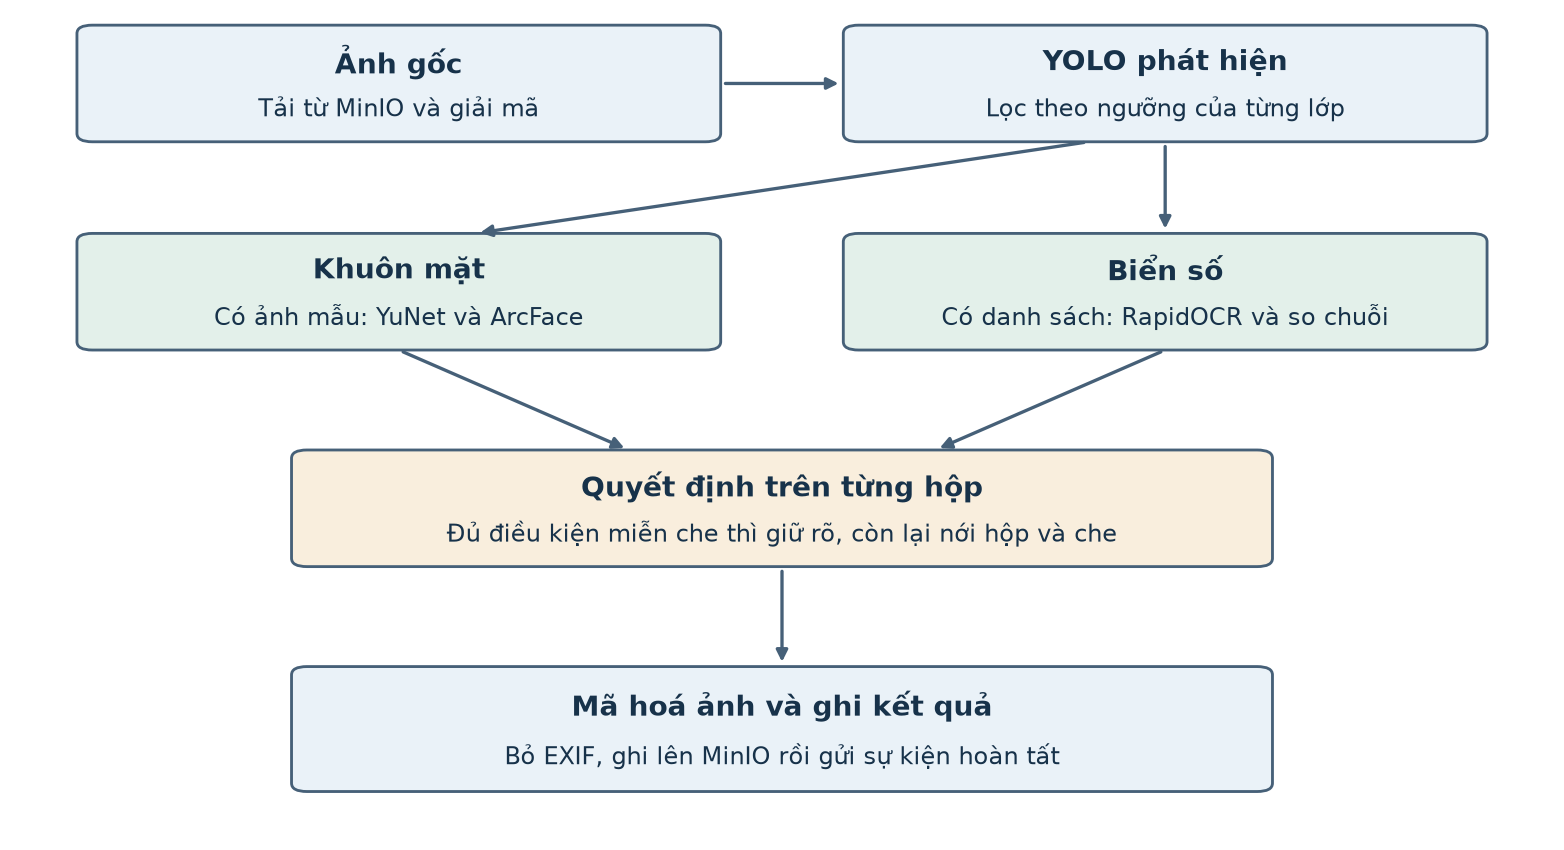
\includegraphics[width=0.95\textwidth]{figures/hinh-3-10-luong-xu-ly-anh.png}
\caption[Luồng xử lý ảnh]{Luồng xử lý ảnh (image-redact). Hai nhánh sau YOLO ứng với khuôn mặt và biển số, chỉ chạy khi có danh sách miễn che}
\label{fig:3-10}
\end{figure}

Ở nhánh khuôn mặt, YuNet căn chỉnh rồi ArcFace so với ảnh mẫu. Ở nhánh biển số, RapidOCR đọc chuỗi rồi so với danh sách. Nguyên tắc chung là mặc định che: điểm tương đồng dưới ngưỡng, OCR không đọc được hay đọc không chắc chắn đều dẫn đến che. Riêng lỗi ở ảnh mẫu, ví dụ ảnh hỏng hoặc không có khuôn mặt, được báo thành lỗi riêng để người dùng biết và thay ảnh.

Với mỗi hộp cần che, vùng che được nới thêm mặc định 10\% mỗi phía. Người dùng chọn làm mờ Gaussian, khảm ô (pixelate) hoặc phủ đen. Độ mạnh được tính theo chiều rộng vùng che, nên khuôn mặt lớn hay nhỏ đều được che như nhau. Ảnh kết quả được mã hoá lại từ điểm ảnh, do đó EXIF và toạ độ GPS của ảnh gốc không còn. Khi người dùng sửa vùng che trên web, hệ thống áp dụng danh sách hộp mới lên ảnh gốc mà không phải chạy lại YOLO.

\textbf{Luồng xử lý video.} Nếu một biển số chỉ đọc rõ ở giữa clip thì quyết định miễn che ngay từ khung đầu sẽ thiếu căn cứ. Vì vậy video được đọc hai lượt: lượt đầu gom bằng chứng trên cả quỹ đạo, lượt sau mới dựng video đầu ra (Hình~\ref{fig:3-11}). Cái giá phải trả là đọc lại video một lần.

\begin{figure}[!htbp]
\centering
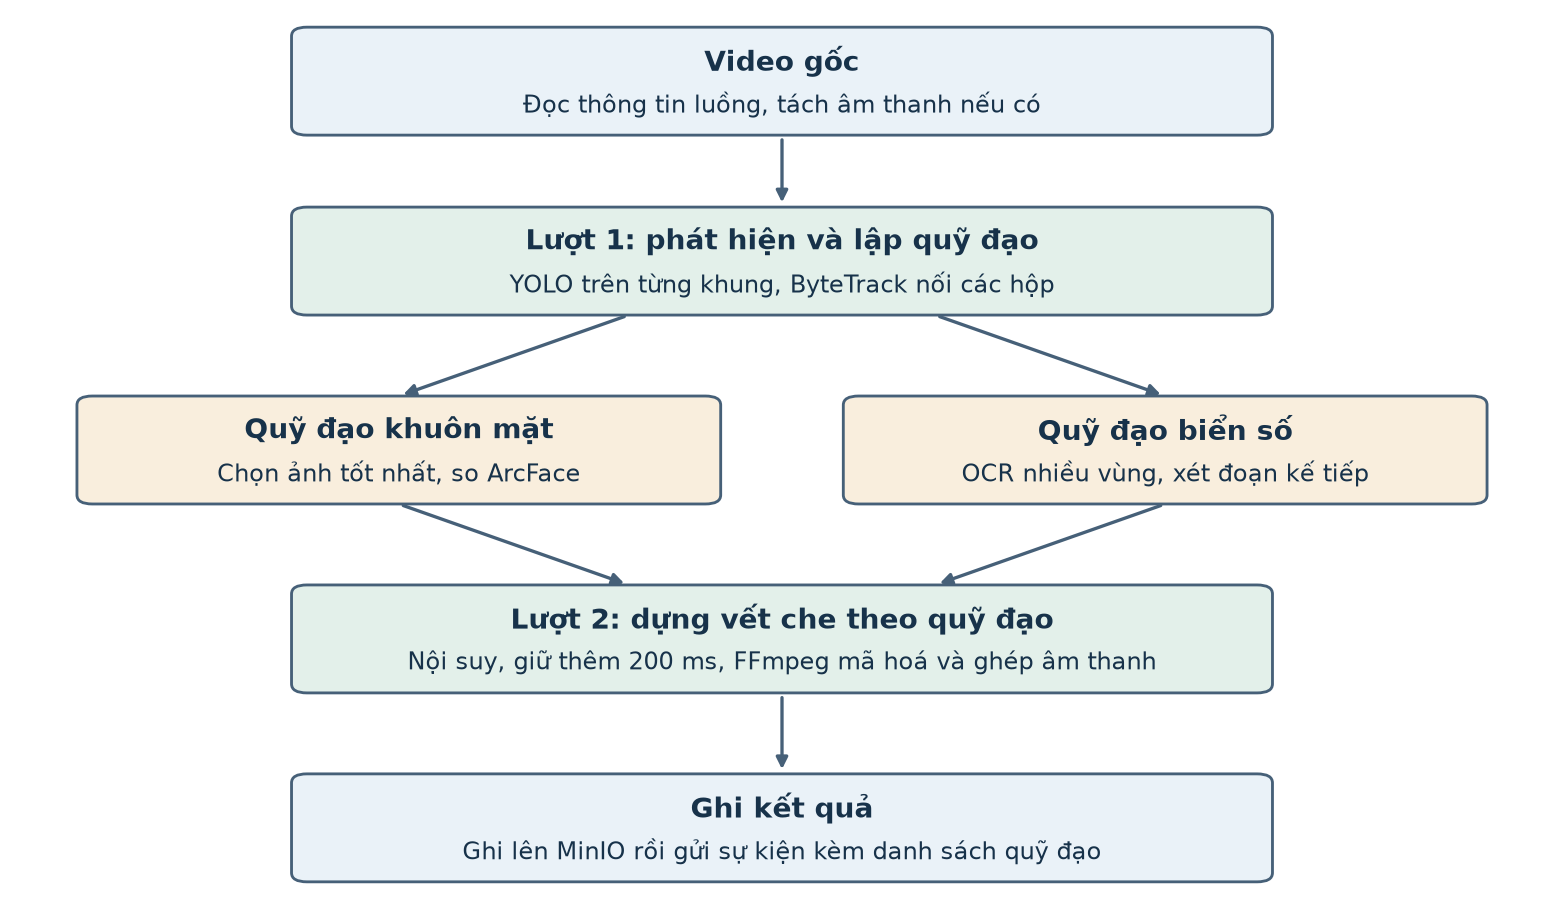
\includegraphics[width=0.95\textwidth]{figures/hinh-3-11-luong-xu-ly-video.png}
\caption[Luồng xử lý video]{Luồng xử lý video (video-redact). Quyết định miễn che nằm giữa lượt theo dõi và lượt dựng video}
\label{fig:3-11}
\end{figure}

Ở lượt đầu, YOLO phát hiện trên từng khung và ByteTrack nối các hộp thành quỹ đạo. Hộp đạt ngưỡng nhưng chưa được cấp mã vẫn được giữ: hệ thống thử ghép với hộp cùng lớp ở khung trước, nếu không được thì cấp mã riêng. Khoảng mất dấu dưới 167 ms được nội suy, còn dài hơn thì tách thành đoạn mới để không nối qua quãng thiếu quan sát. Vết che còn được giữ thêm 200 ms trước và sau mỗi chuỗi phát hiện để không bị nhấp nháy. Hai khoảng thời gian này được đổi ra số khung theo tốc độ của video.

Với khuôn mặt, hệ thống chọn một ảnh tốt nhất của quỹ đạo theo điểm phát hiện, kích thước và độ nét để so với ảnh mẫu. Với biển số, hệ thống đọc ảnh đại diện và tối đa năm vùng cắt rộng nhất, dừng ngay khi khớp. Nếu một biển bị tách thành nhiều đoạn, đoạn nằm gần đoạn đã khớp có thể được kế thừa quyết định, với điều kiện hai đoạn gần nhau về thời gian, vị trí và đoạn đang xét không đọc ra biển khác. Chỉ đoạn khớp OCR trực tiếp mới được làm nguồn kế thừa, nên việc miễn che không lan truyền dây chuyền.

Ở lượt sau, từng khung được đọc lại, áp dụng vết che rồi chuyển cho FFmpeg mã hoá H.264. Âm thanh gốc được ghép lại nguyên vẹn và siêu dữ liệu bị xoá. Cùng với tệp MP4, Backend nhận được thời điểm khung đại diện, các khoảng điểm thấp và các khoảng mất dấu của từng quỹ đạo. Nhờ đó, người dùng có thể nhảy thẳng đến đoạn cần kiểm tra.
